%!TEX TS-program = xelatex
%!TEX encoding = UTF-8 Unicode

\documentclass{harvard-thesis}

% ToDo notes package
\usepackage{packages/todonotes}
\usepackage{array}

% for much better looking tables
\usepackage{booktabs}

\usepackage{multirow}
\usepackage{tabularx}
\usepackage{tabulary}
\usepackage{varwidth}

\usepackage{amsthm}
\usepackage{enumitem}

% package used to draw boxes around environments
\usepackage{mdframed}

% English *and* German are necessary!
\usepackage[german,english]{babel}

\theoremstyle{plain}
\newtheorem{thm}{Theorem}[chapter] % reset theorem numbering for each chapter
\theoremstyle{definition}
\newtheorem{defn}[thm]{Definition} % definition numbers are dependent on theorem numbers
\newtheorem{exmp}[thm]{Example} % same for example numbers
\newtheorem{resques}[thm]{Research Question} % same for research questions
\newtheorem{hypoth}[thm]{Hypothesis} % same for research questions
\newtheorem*{hypoth*}{Hypothesis} % same for research questions

% These commands are defined for new column types in tables.
% Sooner or later you will have some trouble with tables, anyway. :-)
\newcolumntype{M}[1]{>{\begin{varwidth}[t]{#1}}l<{\end{varwidth}}}
\newcolumntype{L}[1]{>{\raggedright\arraybackslash}p{#1}}
\newcolumntype{C}[1]{>{\centering\arraybackslash}p{#1}}
\newcolumntype{R}[1]{>{\raggedleft\arraybackslash}p{#1}}

% If you required that some words should be NEVER be hyphenated,
% then, include them here:
%\hyphenation{PiCsMu}

\begin{document}

% Also, there's the possibility to include commands of terms that are
% used with a high frequency. The advantage of using commands that are
% translated into text is that, if you have to change the terms, then it
% will be automatically reflected to the whole text without any effort!
% You just need to use the commands throughout the thesis, of course.
%
%\newcommand{\picsmu}{PiCsMu}
%\newcommand{\picsmuuser}[1]{\picsmu user#1}
%\newcommand{\picsmuapplication}[1]{\picsmu application}
%\newcommand{\picsmusystem}[1]{\picsmu system}
%\newcommand{\cloud}[1]{Cloud#1}

%\newcommand{\ptopnetwork}[1]{P2P network#1}
%\newcommand{\ptopsystem}[1]{P2P system#1}

%\newcommand{\cloudcomputing}{Cloud computing}
%\newcommand{\cloudservice}[1]{Cloud service#1}
%\newcommand{\cloudprovider}[1]{Cloud provider#1}
%%%%%%%%%%%%%%%%%%%%%%%%%%%%%

% the front matter
% some details about the thesis

\title{IFI-UZH Thesis Template Based on the Harvard Thesis Style}
\author{Guilherme Sperb Machado}
\advisor{Prof. FirstName LastName, Ph.D.}
\coadvisor{Prof. FirstName LastName, Ph.D.}

\approved{November 2015} % month/year of when you presented your thesis
\faculty{Faculty of Business, Economics and Informatics}

\degreeconferralplace{Zurich} % degree conferral place
\degreeconferraldate{June 1, 2016} % degree conferral date/promotionstermin
\chairdoctoralboard{Prof. FirstName LastName, Ph.D.}

% about the university
\department{Faculty of Economics, \\Business Administration And \\Information
Technology}
\university{University of Zurich}
\authorcity{Porto Alegre, RS, Brazil}


% If the title gets too long that the cover is placed to the second page, then, you should adjust the
% "beforeTitle" and "afterTitle" attributes. Setting these attributes overwrite the default values,
% which are 70pt, respectively.
% Example: \coveruzh[beforeTitle=60pt, afterTitle=50pt]
\coveruzh

%\copyrightpage
\frontmatter
\abstractpage
\kurzfassungspage
\tableofcontents
%\authorlist
%\dedicationpage

\vspace*{\fill} \newpage
\setcounter{page}{1}
\pagenumbering{arabic}

\setstretch{1.1}

\mainmatter

\chapter{Introduction}\label{chap:introduction}

\lettrine{P}{ater noster}, qui es in cælis: Sanctificétur nomen tuum: Advéniat regnum tuum: Fiat volúntas tua, sicut in cælo, et in terra. Panem nostrum quotidiánum da nobis hódie: Et dimítte nobis débita nostra, sicut et nos dismíttimus debitóribus nostris. Et ne nos indúcas in tentatiónem. Sed líbera nos a malo. Amen.

\section{Lorem Ipsum Dolor Sit Amet 1}\label{introduction:sec:section_name_1}

Líbera nos, quæsumus, Dómine, ab ómnibus malis, prætéritis, præséntibus, et futúris: et intercedénte beáta et gloriósa semper Vírgine Dei Genitríce María, cum beátis Apóstolis tuis Petro et Paulo, atque Andréa, et ómnibus anctis, + da propítius pacem in diébus nostris: ut ope misericórdiæ tuæ adjúti, et a peccáto simus semper líberi, et ab omni perturbatióne secúri.

\begin{figure}
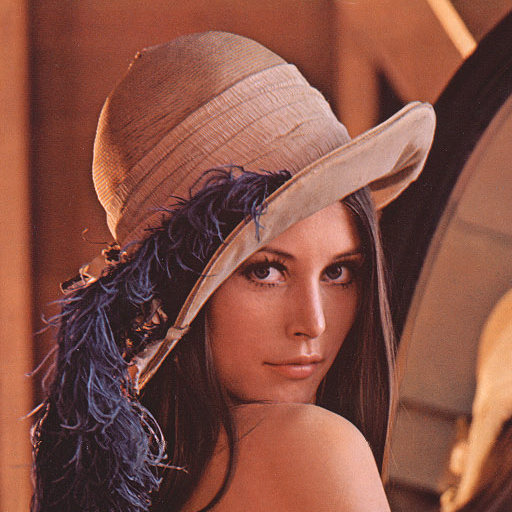
\includegraphics[width=\textwidth]{figs/introduction/lena}
\caption{Lorem ipsum dolor sit amet}
\label{introduction:fig:figure_name_1}
\end{figure}

Dómine Jesu Christe, qui dixísti Apóstolis tuis: Pacem relínquo vobis, pacem meam do vobis: ne respícias peccáta mea, sed fidem Ecclésiæ tuæ; eámque secúndum voluntátem tuam pacificáre et coadunáre dignéris: Qui vivis et regnas Deus per ómnia sæcula sæculórum. Amen. (cf. Figure \ref{introduction:fig:figure_name_1}).

Dómine Jesu Christe, Fili Dei vivi, qui ex voluntáte Patris, cooperánte Spíritu Sancto, per mortem tuam mundum vivificásti: líbera me per hoc sacrosánctum Corpus et Sánguinem tuum ab ómnibus iniquitátibus meis, et univérsis malis: et fac me tuis semper inhærére mandátis, et a te numquam separári permíttas: Qui cum eódem Deo Patre, et Spíritu Sancto vivis et regnas Deus in sæcula sæculórum. Amen.

\section{Lorem Ipsum Dolor Sit Amet 2}\label{introduction:sec:section_name_2}

Percéptio Córporis tui, Dómine Jesu Christe, quod ego indígnus súmere præsúmo, non mihi provéniat in judícium et condemnatiónem: sed pro tua pietáte prosit mihi ad tutaméntum mentis et córporis, et ad medélam percipiéndam: Qui vivis et regnas cum Deo Patre in unitáte Spíritus Sancti Deus, per ómnia sæcula sæculórum. Amen.

Exáudi nos, Dómine sancte, Pater omnípotens, ætérne Deus, et míttere dignéris sanctum Angelum tuum de cælis, qui custódiat, fóveat, prótegat, vísitet, atque deféndat omnes habitántes in hoc habitáculo. Per Christum Dóminum nostrum:
\begin{resques}\label{introduction:sec:section_name_2:resques_1}
Lorem ipsum dolor sit amet, consectetur adipisicing elit, sed do eiusmod tempor incididunt ut labore et dolore magna aliqua.
\end{resques}
\begin{resques}\label{introduction:sec:section_name_2:resques_2}
Lorem ipsum dolor sit amet, consectetur adipisicing elit, sed do eiusmod tempor incididunt ut labore et dolore magna aliqua.
\end{resques}
\begin{resques}\label{introduction:sec:section_name_2:resques_3}
Lorem ipsum dolor sit amet, consectetur adipisicing elit, sed do eiusmod tempor incididunt ut labore et dolore magna aliqua.
\end{resques}

Vidi aquam egrediéntem de templo, a látere dextro, allelúia: et omnes ad quos pervénit aqua ista salvi facti sunt et dicent: allelúia, allelúia.

Lorem ipsum dolor sit amet, consectetur adipisicing elit, sed do eiusmod tempor incididunt ut labore et dolore magna aliqua. Ut enim ad minim veniam, quis nostrud exercitation ullamco laboris nisi ut aliquip ex ea commodo consequat. Duis aute irure dolor in reprehenderit in voluptate velit esse cillum dolore eu fugiat nulla pariatur. Excepteur sint occaecat cupidatat non proident, sunt in culpa qui officia deserunt mollit anim id est laborum.

\section{Lorem Ipsum Dolor Sit Amet 3}\label{introduction:sec:section_name_3}

Júdica me, Deus, et discérne causam meam de gente non sancta: ab hómine iníquo, et dolóso érue me. Quia tu es, Deus, fortitúdo mea: quare me repulísti, et quare tristis incédo, dum afflígit me inimícus? Emítte lucem tuam, et veritátem tuam: ipsa me deduxérunt, et aduxérunt in montem sanctum tuum, et in tabernácula tua. Et introíbo ad altáre Dei: ad Deum qui lætíficat juventútem meam. Confitébor tibi in cíthara, Deus, Deus meus: quare tristis es, ánima mea, et quare contúrbas me? Spera in Deo, quóniam adhuc confitébor illi: salutáre vultus mei, et Deus meus. Glória Patri, et Fílio, et Spirítui Sancto. Sicut erat in princípio et nunc, et semper, et in sæcula sæculórum. Amen.

Lorem ipsum dolor sit amet, consectetur adipisicing elit, sed do eiusmod tempor incididunt ut labore et dolore magna aliqua. Ut enim ad minim veniam, quis nostrud exercitation ullamco laboris nisi ut aliquip ex ea commodo consequat. Duis aute irure dolor in reprehenderit in voluptate velit esse cillum dolore eu fugiat nulla pariatur. Excepteur sint occaecat cupidatat non proident, sunt in culpa qui officia deserunt mollit anim id est laborum.

\section{Thesis Contributions}\label{introduction:sec:contributions}

Lorem ipsum dolor sit amet, consectetur adipisicing elit, sed do eiusmod tempor incididunt ut labore et dolore magna aliqua. Ut enim ad minim veniam, quis nostrud exercitation ullamco laboris nisi ut aliquip ex ea commodo consequat. Duis aute irure dolor in reprehenderit in voluptate velit esse cillum dolore eu fugiat nulla pariatur. Excepteur sint occaecat cupidatat non proident, sunt in culpa qui officia deserunt mollit anim id est laborum:

\begin{enumerate}
  
  \item Lorem ipsum dolor sit amet, consectetur adipisicing elit, sed do eiusmod tempor incididunt ut labore et dolore magna aliqua. Ut enim ad minim veniam, quis nostrud exercitation ullamco laboris nisi ut aliquip ex ea commodo consequat. Duis aute irure dolor in reprehenderit in voluptate velit esse cillum dolore eu fugiat nulla pariatur. Excepteur sint occaecat cupidatat non proident, sunt in culpa qui officia deserunt mollit anim id est laborum;
  
  \item Lorem ipsum dolor sit amet, consectetur adipisicing elit, sed do eiusmod tempor incididunt ut labore et dolore magna aliqua. Ut enim ad minim veniam, quis nostrud exercitation ullamco laboris nisi ut aliquip ex ea commodo consequat. Duis aute irure dolor in reprehenderit in voluptate velit esse cillum dolore eu fugiat nulla pariatur. Excepteur sint occaecat cupidatat non proident, sunt in culpa qui officia deserunt mollit anim id est laborum;
  
  \item Lorem ipsum dolor sit amet, consectetur adipisicing elit, sed do eiusmod tempor incididunt ut labore et dolore magna aliqua. Ut enim ad minim veniam, quis nostrud exercitation ullamco laboris nisi ut aliquip ex ea commodo consequat. Duis aute irure dolor in reprehenderit in voluptate velit esse cillum dolore eu fugiat nulla pariatur. Excepteur sint occaecat cupidatat non proident, sunt in culpa qui officia deserunt mollit anim id est laborum;
  
  \item Lorem ipsum dolor sit amet, consectetur adipisicing elit, sed do eiusmod tempor incididunt ut labore et dolore magna aliqua. Ut enim ad minim veniam, quis nostrud exercitation ullamco laboris nisi ut aliquip ex ea commodo consequat. Duis aute irure dolor in reprehenderit in voluptate velit esse cillum dolore eu fugiat nulla pariatur. Excepteur sint occaecat cupidatat non proident, sunt in culpa qui officia deserunt mollit anim id est laborum.
  
\end{enumerate}

\section{Thesis Outline}\label{introduction:sec:thesis_outline}

Lorem ipsum dolor sit amet, consectetur adipisicing elit, sed do eiusmod tempor incididunt ut labore et dolore magna aliqua. Ut enim ad minim veniam, quis nostrud exercitation ullamco laboris nisi ut aliquip ex ea commodo consequat. Duis aute irure dolor in reprehenderit in voluptate velit esse cillum dolore eu fugiat nulla pariatur. Excepteur sint occaecat cupidatat non proident, sunt in culpa qui officia deserunt mollit anim id est laborum.

Chapter \ref{chap:introduction} lorem ipsum dolor sit amet, consectetur adipisicing elit, sed do eiusmod tempor incididunt ut labore et dolore magna aliqua. Ut enim ad minim veniam, quis nostrud exercitation ullamco laboris nisi ut aliquip ex ea commodo consequat. Duis aute irure dolor in reprehenderit in voluptate velit esse cillum dolore eu fugiat nulla pariatur. Excepteur sint occaecat cupidatat non proident, sunt in culpa qui officia deserunt mollit anim id est laborum.

Lorem ipsum dolor sit amet, consectetur adipisicing elit, sed do eiusmod tempor incididunt ut labore et dolore magna aliqua. Ut enim ad minim veniam, quis nostrud exercitation ullamco laboris nisi ut aliquip ex ea commodo consequat. Duis aute irure dolor in reprehenderit in voluptate velit esse cillum dolore eu fugiat nulla pariatur. Excepteur sint occaecat cupidatat non proident, sunt in culpa qui officia deserunt mollit anim id est laborum -- cf. Chapter \ref{chap:related_work}.

Chapter \ref{chap:solution_design} lorem ipsum dolor sit amet, consectetur adipisicing elit, sed do eiusmod tempor incididunt ut labore et dolore magna aliqua. Ut enim ad minim veniam, quis nostrud exercitation ullamco laboris nisi ut aliquip ex ea commodo consequat. Duis aute irure dolor in reprehenderit in voluptate velit esse cillum dolore eu fugiat nulla pariatur. Excepteur sint occaecat cupidatat non proident, sunt in culpa qui officia deserunt mollit anim id est laborum.

\chapter{Terminology and Related Work}\label{chap:related_work}

\lettrine{L}{orem} ipsum dolor sit amet, consectetur adipisicing elit, sed do eiusmod tempor incididunt ut labore et dolore magna aliqua. Ut enim ad minim veniam, quis nostrud exercitation ullamco laboris nisi ut aliquip ex ea commodo consequat. Duis aute irure dolor in reprehenderit in voluptate velit esse cillum dolore eu fugiat nulla pariatur. Excepteur sint occaecat cupidatat non proident, sunt in culpa qui officia deserunt mollit anim id est laborum.

\section{Terminology}\label{related_work:sec:terminology}

Lorem ipsum dolor sit amet, consectetur adipisicing elit, sed do eiusmod tempor incididunt ut labore et dolore magna aliqua. Ut enim ad minim veniam, quis nostrud exercitation ullamco laboris nisi ut aliquip ex ea commodo consequat. Duis aute irure dolor in reprehenderit in voluptate velit esse cillum dolore eu fugiat nulla pariatur. Excepteur sint occaecat cupidatat non proident, sunt in culpa qui officia deserunt mollit anim id est laborum -- cf. Figure \ref{related_work:fig:figure_name_1}.

\begin{defn}
\em
``Lorem ipsum dolor sit amet, consectetur adipisicing elit, sed do eiusmod tempor incididunt ut labore et dolore magna aliqua. Ut enim ad minim veniam, quis nostrud exercitation ullamco laboris nisi ut aliquip ex ea commodo consequat. Duis aute irure dolor in reprehenderit in voluptate velit esse cillum dolore eu fugiat nulla pariatur. Excepteur sint occaecat cupidatat non proident, sunt in culpa qui officia deserunt mollit anim id est laborum'' \cite{rfc1}
\end{defn}

\begin{defn}
\em
Lorem ipsum dolor sit amet, consectetur adipisicing elit, sed do eiusmod tempor incididunt ut labore et dolore magna aliqua. Ut enim ad minim veniam, quis nostrud exercitation ullamco laboris nisi ut aliquip ex ea commodo consequat. Duis aute irure dolor in reprehenderit in voluptate velit esse cillum dolore eu fugiat nulla pariatur. Excepteur sint occaecat cupidatat non proident, sunt in culpa qui officia deserunt mollit anim id est laborum \cite{rfc666}.
\end{defn}

\begin{figure}[h]
\centering
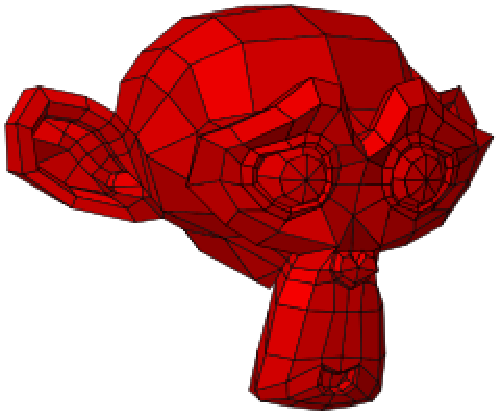
\includegraphics[width=0.6\textwidth]{figs/chapter2/suzanne}
\caption{Lorem ipsum dolor sit amet}
\label{related_work:fig:figure_name_1}
\end{figure}

\section{Lorem Ipsum Dolor Sit Amet}\label{related_work:sec:section_2}

Lorem ipsum dolor sit amet, consectetur adipisicing elit, sed do eiusmod tempor incididunt ut labore et dolore magna aliqua. Ut enim ad minim veniam, quis nostrud exercitation ullamco laboris nisi ut aliquip ex ea commodo consequat. Duis aute irure dolor in reprehenderit in voluptate velit esse cillum dolore eu fugiat nulla pariatur. Excepteur sint occaecat cupidatat non proident, sunt in culpa qui officia deserunt mollit anim id est laborum -- cf. Table \ref{related_work:tab:table_name_1} and \ref{related_work:tab:table_name_2}.

\begin{table}[htb]
\centering
\renewcommand{\arraystretch}{1.0}
\caption{Lorem ipsum dolor sit amet}
\label{related_work:tab:table_name_1}
\begin{tabular}{clccc}
\toprule
\multicolumn{2}{c}{\multirow{2}{*}[-2em]{\begin{tabular}[c]{@{}c@{}}Just Example\\Table\end{tabular}}} & \multicolumn{3}{c}{Example Blah}                                                                                                                                                                                                           \\ \cmidrule{3-5}
& \multicolumn{1}{c}{} & \multicolumn{1}{c}{\begin{tabular}[c]{@{}c@{}}\textbf{Blah}\\\textbf{Bloh}\end{tabular}} & \multicolumn{1}{c}{\begin{tabular}[c]{@{}c@{}}\textbf{Blah}\\\textbf{Bluh}\\\textbf{Reliability}\end{tabular}} & \multicolumn{1}{c}{\begin{tabular}[c]{@{}c@{}}\textbf{Blah}\\\textbf{Blih}\\\textbf{Bluh}\end{tabular}} \\ \midrule
\multicolumn{1}{c}{\multirow{7}{*}[-1em]{\rotatebox[origin=c]{90}{Some Stuff}}} & \textbf{One} & No & No & No \\ \cmidrule{2-5}
& \textbf{Two} & No & No & No \\ \cmidrule{2-5}
& \textbf{Three} & No & No & No \\ \cmidrule{2-5}
& \textbf{Four} & No & No & No \\ \cmidrule{2-5}
& \textbf{Five} & Yes & No & No \\ \cmidrule{2-5}
& \textbf{Six} & Yes & Yes & No \\ \cmidrule{2-5}
& \textbf{Seven} & Yes & No & No \\ \midrule
\multicolumn{1}{c}{\multirow{8}{*}[-1em]{\rotatebox[origin=c]{90}{Other Stuff}}} & \textbf{Eight} & No & No & No \\ \cmidrule{2-5}
& \textbf{Night} & No & No & No \\ \cmidrule{2-5}
& \textbf{Ten} & No & No & No \\ \cmidrule{2-5}
& \textbf{Eleven} & No & No & No \\ \cmidrule{2-5}
& \textbf{Twelve} & No & No & No \\ \cmidrule{2-5}
& \textbf{Thirteen} & No & No & No \\ \cmidrule{2-5}
& \textbf{Fourteen} & No & No & No \\ \cmidrule{2-5}
& \textbf{Fifthteen} & No & No & No \\ \midrule\midrule
\multicolumn{2}{c}{\textbf{Sixteen}} & Yes & Yes & Yes \\ \bottomrule
\end{tabular}
\end{table}

Lorem ipsum dolor sit amet, consectetur adipisicing elit, sed do eiusmod tempor incididunt ut labore et dolore magna aliqua. Ut enim ad minim veniam, quis nostrud exercitation ullamco laboris nisi ut aliquip ex ea commodo consequat. Duis aute irure dolor in reprehenderit in voluptate velit esse cillum dolore eu fugiat nulla pariatur. Excepteur sint occaecat cupidatat non proident, sunt in culpa qui officia deserunt mollit anim id est laborum.

\begin{table}[htb]
\centering
\renewcommand{\arraystretch}{1.1}
\caption{Lorem ipsum dolor sit amet}
\label{related_work:tab:table_name_2}
\begin{tabular}{lccccccc||c}
\toprule
 & \multicolumn{8}{c}{Just an example}
\\ \cmidrule{2-9}
\multicolumn{1}{c}{\multirow{2}{*}[+2em]{Parameters}} & \rotatebox[origin=c]{90}{\textbf{One}} & \rotatebox[origin=c]{90}{\textbf{Two}} & \rotatebox[origin=c]{90}{\textbf{Three}} & \rotatebox[origin=c]{90}{\textbf{Four}} & \rotatebox[origin=c]{90}{\textbf{Five}} & \rotatebox[origin=c]{90}{\textbf{Six}} & \rotatebox[origin=c]{90}{\textbf{Seven}} & \rotatebox[origin=c]{90}{\textbf{Eight}} \\ \midrule
\begin{tabular}[c]{@{}l@{}}Parameter Blah\end{tabular}                                                  & No                                 & No                                      & No                                   & No                                     & No                                   & Yes & No & Yes                                 \\ \midrule
\begin{tabular}[c]{@{}l@{}}Parameter\\Blah Bloh\end{tabular}                                                                                                      & No                                 & No                                      & No                                   & No                                     & No                                     & Yes & No & Yes                                 \\ \midrule
\begin{tabular}[c]{@{}l@{}}Parameter\\Blah Blih\end{tabular}                         & Yes                                & Yes                                     & Yes                                  & Yes                                    & Yes                                    & Yes & Yes & Yes                                 \\ \midrule
\begin{tabular}[c]{@{}l@{}}Parameter\\Blah Bluh\end{tabular}                   & Yes                                & No                                      & No                                   & Yes                                    & No                                     & Yes & Yes & Yes                                 \\ \midrule
\begin{tabular}[c]{@{}l@{}}Parameter\\Blah Bloh\end{tabular} & No                                 & No                                      & No                                   & No                                     & Yes                                     & No & No & Yes                                  \\ \midrule
\begin{tabular}[c]{@{}l@{}}Parameter\\Blah Bloh\\Bluh Blih\end{tabular}                                                  & No                                 & No                                      & No                                   & No                                     & No                                     & Yes & No & Yes                                 \\ \midrule
\begin{tabular}[c]{@{}l@{}}Parameter Blih\\Bloh\end{tabular}                                                                                                           & Yes                                & Yes                                     & Yes                                  & Yes                                    & Yes                                    & Yes & Yes & Yes                                 \\ \midrule
\begin{tabular}[c]{@{}l@{}}Parameter Blih\end{tabular}                                                                                                           & No                                 & No                                      & No                                   & No                                     & No                                     & No & No & Yes                                 \\ \bottomrule
\end{tabular}
\end{table}

Lorem ipsum dolor sit amet, consectetur adipisicing elit, sed do eiusmod tempor incididunt ut labore et dolore magna aliqua. Ut enim ad minim veniam, quis nostrud exercitation ullamco laboris nisi ut aliquip ex ea commodo consequat. Duis aute irure dolor in reprehenderit in voluptate velit esse cillum dolore eu fugiat nulla pariatur. Excepteur sint occaecat cupidatat non proident, sunt in culpa qui officia deserunt mollit anim id est laborum.

\chapter{Solution Design}\label{chap:solution_design}

\lettrine{L}{orem ipsum} dolor sit amet, consectetur adipisicing elit, sed do eiusmod tempor incididunt ut labore et dolore magna aliqua. Ut enim ad minim veniam, quis nostrud exercitation ullamco laboris nisi ut aliquip ex ea commodo consequat. Duis aute irure dolor in reprehenderit in voluptate velit esse cillum dolore eu fugiat nulla pariatur. Excepteur sint occaecat cupidatat non proident, sunt in culpa qui officia deserunt mollit anim id est laborum.

Lorem ipsum dolor sit amet, consectetur adipisicing elit, sed do eiusmod tempor incididunt ut labore et dolore magna aliqua. Ut enim ad minim veniam, quis nostrud exercitation ullamco laboris nisi ut aliquip ex ea commodo consequat. Duis aute irure dolor in reprehenderit in voluptate velit esse cillum dolore eu fugiat nulla pariatur. Excepteur sint occaecat cupidatat non proident, sunt in culpa qui officia deserunt mollit anim id est laborum.

\section{Design Objectives}\label{solution_design:sec:design_objectives}

Lorem ipsum dolor sit amet, consectetur adipisicing elit, sed do eiusmod tempor incididunt ut labore et dolore magna aliqua. Ut enim ad minim veniam, quis nostrud exercitation ullamco laboris nisi ut aliquip ex ea commodo consequat. Duis aute irure dolor in reprehenderit in voluptate velit esse cillum dolore eu fugiat nulla pariatur. Excepteur sint occaecat cupidatat non proident, sunt in culpa qui officia deserunt mollit anim id est laborum.

Lorem ipsum dolor sit amet, consectetur adipisicing elit, sed do eiusmod tempor incididunt ut labore et dolore magna aliqua. Ut enim ad minim veniam, quis nostrud exercitation ullamco laboris nisi ut aliquip ex ea commodo consequat. Duis aute irure dolor in reprehenderit in voluptate velit esse cillum dolore eu fugiat nulla pariatur. Excepteur sint occaecat cupidatat non proident, sunt in culpa qui officia deserunt mollit anim id est laborum.

Lorem ipsum dolor sit amet, consectetur adipisicing elit, sed do eiusmod tempor incididunt ut labore et dolore magna aliqua. Ut enim ad minim veniam, quis nostrud exercitation ullamco laboris nisi ut aliquip ex ea commodo consequat. Duis aute irure dolor in reprehenderit in voluptate velit esse cillum dolore eu fugiat nulla pariatur. Excepteur sint occaecat cupidatat non proident, sunt in culpa qui officia deserunt mollit anim id est laborum.

\subsection{Lorem Ipsum Dolor Sit Amet}\label{solution_design:sec:design_objectives:subsec:subsection_name_1}

Lorem ipsum dolor sit amet, consectetur adipisicing elit, sed do eiusmod tempor incididunt ut labore et dolore magna aliqua. Ut enim ad minim veniam, quis nostrud exercitation ullamco laboris nisi ut aliquip ex ea commodo consequat. Duis aute irure dolor in reprehenderit in voluptate velit esse cillum dolore eu fugiat nulla pariatur. Excepteur sint occaecat cupidatat non proident, sunt in culpa qui officia deserunt mollit anim id est laborum.

Lorem ipsum dolor sit amet, consectetur adipisicing elit, sed do eiusmod tempor incididunt ut labore et dolore magna aliqua. Ut enim ad minim veniam, quis nostrud exercitation ullamco laboris nisi ut aliquip ex ea commodo consequat. Duis aute irure dolor in reprehenderit in voluptate velit esse cillum dolore eu fugiat nulla pariatur. Excepteur sint occaecat cupidatat non proident, sunt in culpa qui officia deserunt mollit anim id est laborum.

Lorem ipsum dolor sit amet, consectetur adipisicing elit, sed do eiusmod tempor incididunt ut labore et dolore magna aliqua. Ut enim ad minim veniam, quis nostrud exercitation ullamco laboris nisi ut aliquip ex ea commodo consequat. Duis aute irure dolor in reprehenderit in voluptate velit esse cillum dolore eu fugiat nulla pariatur. Excepteur sint occaecat cupidatat non proident, sunt in culpa qui officia deserunt mollit anim id est laborum.


\chapter{Summary and Conclusions}\label{chap:summary_conclusions}

\lettrine{L}{orem ipsum} dolor sit amet, consectetur adipisicing elit, sed do eiusmod tempor incididunt ut labore et dolore magna aliqua. Ut enim ad minim veniam, quis nostrud exercitation ullamco laboris nisi ut aliquip ex ea commodo consequat. Duis aute irure dolor in reprehenderit in voluptate velit esse cillum dolore eu fugiat nulla pariatur. Excepteur sint occaecat cupidatat non proident, sunt in culpa qui officia deserunt mollit anim id est laborum.

Lorem ipsum dolor sit amet, consectetur adipisicing elit, sed do eiusmod tempor incididunt ut labore et dolore magna aliqua. Ut enim ad minim veniam, quis nostrud exercitation ullamco laboris nisi ut aliquip ex ea commodo consequat. Duis aute irure dolor in reprehenderit in voluptate velit esse cillum dolore eu fugiat nulla pariatur. Excepteur sint occaecat cupidatat non proident, sunt in culpa qui officia deserunt mollit anim id est laborum.

\section{Review of Contributions}\label{summary_conclusions:sec:review_contributions}

Lorem ipsum dolor sit amet, consectetur adipisicing elit, sed do eiusmod tempor incididunt ut labore et dolore magna aliqua. Ut enim ad minim veniam, quis nostrud exercitation ullamco laboris nisi ut aliquip ex ea commodo consequat. Duis aute irure dolor in reprehenderit in voluptate velit esse cillum dolore eu fugiat nulla pariatur. Excepteur sint occaecat cupidatat non proident, sunt in culpa qui officia deserunt mollit anim id est laborum.

\paragraph*{Research Question \ref{introduction:sec:section_name_2:resques_1}:} \textit{Lorem ipsum dolor sit amet, consectetur adipisicing elit, sed do eiusmod tempor incididunt ut labore et dolore magna aliqua?}

Lorem ipsum dolor sit amet, consectetur adipisicing elit, sed do eiusmod tempor incididunt ut labore et dolore magna aliqua. Ut enim ad minim veniam, quis nostrud exercitation ullamco laboris nisi ut aliquip ex ea commodo consequat. Duis aute irure dolor in reprehenderit in voluptate velit esse cillum dolore eu fugiat nulla pariatur. Excepteur sint occaecat cupidatat non proident, sunt in culpa qui officia deserunt mollit anim id est laborum.

Lorem ipsum dolor sit amet, consectetur adipisicing elit, sed do eiusmod tempor incididunt ut labore et dolore magna aliqua. Ut enim ad minim veniam, quis nostrud exercitation ullamco laboris nisi ut aliquip ex ea commodo consequat. Duis aute irure dolor in reprehenderit in voluptate velit esse cillum dolore eu fugiat nulla pariatur. Excepteur sint occaecat cupidatat non proident, sunt in culpa qui officia deserunt mollit anim id est laborum.

\paragraph*{Research Question \ref{introduction:sec:section_name_2:resques_2}:} \textit{Lorem ipsum dolor sit amet, consectetur adipisicing elit, sed do eiusmod tempor incididunt ut labore et dolore magna aliqua?}

Lorem ipsum dolor sit amet, consectetur adipisicing elit, sed do eiusmod tempor incididunt ut labore et dolore magna aliqua. Ut enim ad minim veniam, quis nostrud exercitation ullamco laboris nisi ut aliquip ex ea commodo consequat. Duis aute irure dolor in reprehenderit in voluptate velit esse cillum dolore eu fugiat nulla pariatur. Excepteur sint occaecat cupidatat non proident, sunt in culpa qui officia deserunt mollit anim id est laborum.

Lorem ipsum dolor sit amet, consectetur adipisicing elit, sed do eiusmod tempor incididunt ut labore et dolore magna aliqua. Ut enim ad minim veniam, quis nostrud exercitation ullamco laboris nisi ut aliquip ex ea commodo consequat. Duis aute irure dolor in reprehenderit in voluptate velit esse cillum dolore eu fugiat nulla pariatur. Excepteur sint occaecat cupidatat non proident, sunt in culpa qui officia deserunt mollit anim id est laborum.

\paragraph*{Research Question \ref{introduction:sec:section_name_2:resques_3}:} \textit{Lorem ipsum dolor sit amet, consectetur adipisicing elit, sed do eiusmod tempor incididunt ut labore et dolore magna aliqua?}

Lorem ipsum dolor sit amet, consectetur adipisicing elit, sed do eiusmod tempor incididunt ut labore et dolore magna aliqua. Ut enim ad minim veniam, quis nostrud exercitation ullamco laboris nisi ut aliquip ex ea commodo consequat. Duis aute irure dolor in reprehenderit in voluptate velit esse cillum dolore eu fugiat nulla pariatur. Excepteur sint occaecat cupidatat non proident, sunt in culpa qui officia deserunt mollit anim id est laborum.

Lorem ipsum dolor sit amet, consectetur adipisicing elit, sed do eiusmod tempor incididunt ut labore et dolore magna aliqua. Ut enim ad minim veniam, quis nostrud exercitation ullamco laboris nisi ut aliquip ex ea commodo consequat. Duis aute irure dolor in reprehenderit in voluptate velit esse cillum dolore eu fugiat nulla pariatur. Excepteur sint occaecat cupidatat non proident, sunt in culpa qui officia deserunt mollit anim id est laborum.

\section{General Conclusions}\label{summary_conclusions:sec:general_conclusions}

Dóminus vobíscum. Inítium sancti Evangélii secúndum Joánnem. In princípio erat Verbum, et Verbum erat apud Deum, et Deus erat Verbum. Hoc erat in princípio apud Deum. Omnia per ipsum facta sunt: et sine ipso factum est nihil, quod factum est: in ipso vita erat, et viat erat lux hóminum: et lux in ténebris lucet, et ténebræ eam non comprehendérunt. Fuit homo missus a Deo, cui nomen erat Joánnes. Hic venit in testimónium, ut testimónium perhibéret de lúmine, ut omnes créderent per illum. Non erat ille lux, sed ut testimónium perhibéret de lúmine. Erat lux vera, quæ illúminat omnem hóminem veniéntem in hunc mundum. In mundo erat, et mundus per ipsum factus est, et mundus eum non cognóvit. In própria venit, et sui eum non recepérunt. Quotquot autem recepérunt eum, dedit eis potestátem fílios Dei fíeri, his, qui credunt in nómine ejus: qui non ex sanguínibus, neque ex voluntáte carnis, neque ex voluntáte viri, sed ex Deo nati sunt. Genuflect ET VERBUM CARO FACTUM EST, et habitávit in nobis: et vídimus glóriam ejus, glóriam quasi Unigéniti a Patre, plenum grátiæ et veritátis. Deo grátias -- cf. Figure \ref{summary_conclusions:fig:figure_name_1}.

\begin{figure}
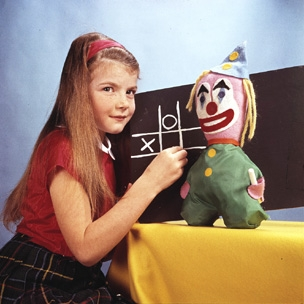
\includegraphics[width=\textwidth]{figs/chapterN/TCF_centre}
\caption{Lorem ipsum dolor sit amet}
\label{summary_conclusions:fig:figure_name_1}
\end{figure}

Lorem ipsum dolor sit amet, consectetur adipisicing elit, sed do eiusmod tempor incididunt ut labore et dolore magna aliqua. Ut enim ad minim veniam, quis nostrud exercitation ullamco laboris nisi ut aliquip ex ea commodo consequat. Duis aute irure dolor in reprehenderit in voluptate velit esse cillum dolore eu fugiat nulla pariatur. Excepteur sint occaecat cupidatat non proident, sunt in culpa qui officia deserunt mollit anim id est laborum.

Lorem ipsum dolor sit amet, consectetur adipisicing elit, sed do eiusmod tempor incididunt ut labore et dolore magna aliqua. Ut enim ad minim veniam, quis nostrud exercitation ullamco laboris nisi ut aliquip ex ea commodo consequat. Duis aute irure dolor in reprehenderit in voluptate velit esse cillum dolore eu fugiat nulla pariatur. Excepteur sint occaecat cupidatat non proident, sunt in culpa qui officia deserunt mollit anim id est laborum.

Lorem ipsum dolor sit amet, consectetur adipisicing elit, sed do eiusmod tempor incididunt ut labore et dolore magna aliqua. Ut enim ad minim veniam, quis nostrud exercitation ullamco laboris nisi ut aliquip ex ea commodo consequat. Duis aute irure dolor in reprehenderit in voluptate velit esse cillum dolore eu fugiat nulla pariatur. Excepteur sint occaecat cupidatat non proident, sunt in culpa qui officia deserunt mollit anim id est laborum.

\section{Future Work}\label{summary_conclusions:sec:future_work}

Lorem ipsum dolor sit amet, consectetur adipisicing elit, sed do eiusmod tempor incididunt ut labore et dolore magna aliqua. Ut enim ad minim veniam, quis nostrud exercitation ullamco laboris nisi ut aliquip ex ea commodo consequat. Duis aute irure dolor in reprehenderit in voluptate velit esse cillum dolore eu fugiat nulla pariatur. Excepteur sint occaecat cupidatat non proident, sunt in culpa qui officia deserunt mollit anim id est laborum.

Lorem ipsum dolor sit amet, consectetur adipisicing elit, sed do eiusmod tempor incididunt ut labore et dolore magna aliqua. Ut enim ad minim veniam, quis nostrud exercitation ullamco laboris nisi ut aliquip ex ea commodo consequat. Duis aute irure dolor in reprehenderit in voluptate velit esse cillum dolore eu fugiat nulla pariatur. Excepteur sint occaecat cupidatat non proident, sunt in culpa qui officia deserunt mollit anim id est laborum.

Lorem ipsum dolor sit amet, consectetur adipisicing elit, sed do eiusmod tempor incididunt ut labore et dolore magna aliqua. Ut enim ad minim veniam, quis nostrud exercitation ullamco laboris nisi ut aliquip ex ea commodo consequat. Duis aute irure dolor in reprehenderit in voluptate velit esse cillum dolore eu fugiat nulla pariatur. Excepteur sint occaecat cupidatat non proident, sunt in culpa qui officia deserunt mollit anim id est laborum.

Lorem ipsum dolor sit amet, consectetur adipisicing elit, sed do eiusmod tempor incididunt ut labore et dolore magna aliqua. Ut enim ad minim veniam, quis nostrud exercitation ullamco laboris nisi ut aliquip ex ea commodo consequat. Duis aute irure dolor in reprehenderit in voluptate velit esse cillum dolore eu fugiat nulla pariatur. Excepteur sint occaecat cupidatat non proident, sunt in culpa qui officia deserunt mollit anim id est laborum.

\singlespacing
\backmatter

% The cleardoublepage and phantomsection commands are needed because
% the "Reference" chapter was wrong in the index hyperlinks
% Now, it's correct.
\cleardoublepage\phantomsection

% the back matter
\clearpage
\addcontentsline{toc}{chapter}{References}

{\small
\setstretch{1.1}
\bibliography{bib/rfc}}

\bibliographystyle{amsplain}

\appendix

\chapter{Appendix}
%\addcontentsline{toc}{chapter}{Appendix}
\label{chap:appendix}

\section{Lorem ipsum dolor sit amet}\label{appendix:sec:section_name_1}

Lorem ipsum dolor sit amet, consectetur adipisicing elit, sed do eiusmod tempor incididunt ut labore et dolore magna aliqua. Ut enim ad minim veniam, quis nostrud exercitation ullamco laboris nisi ut aliquip ex ea commodo consequat. Duis aute irure dolor in reprehenderit in voluptate velit esse cillum dolore eu fugiat nulla pariatur. Excepteur sint occaecat cupidatat non proident, sunt in culpa qui officia deserunt mollit anim id est laborum (cf. Figure \ref{appendix:fig:utah_teapot}).

\begin{figure}[h]
\centering
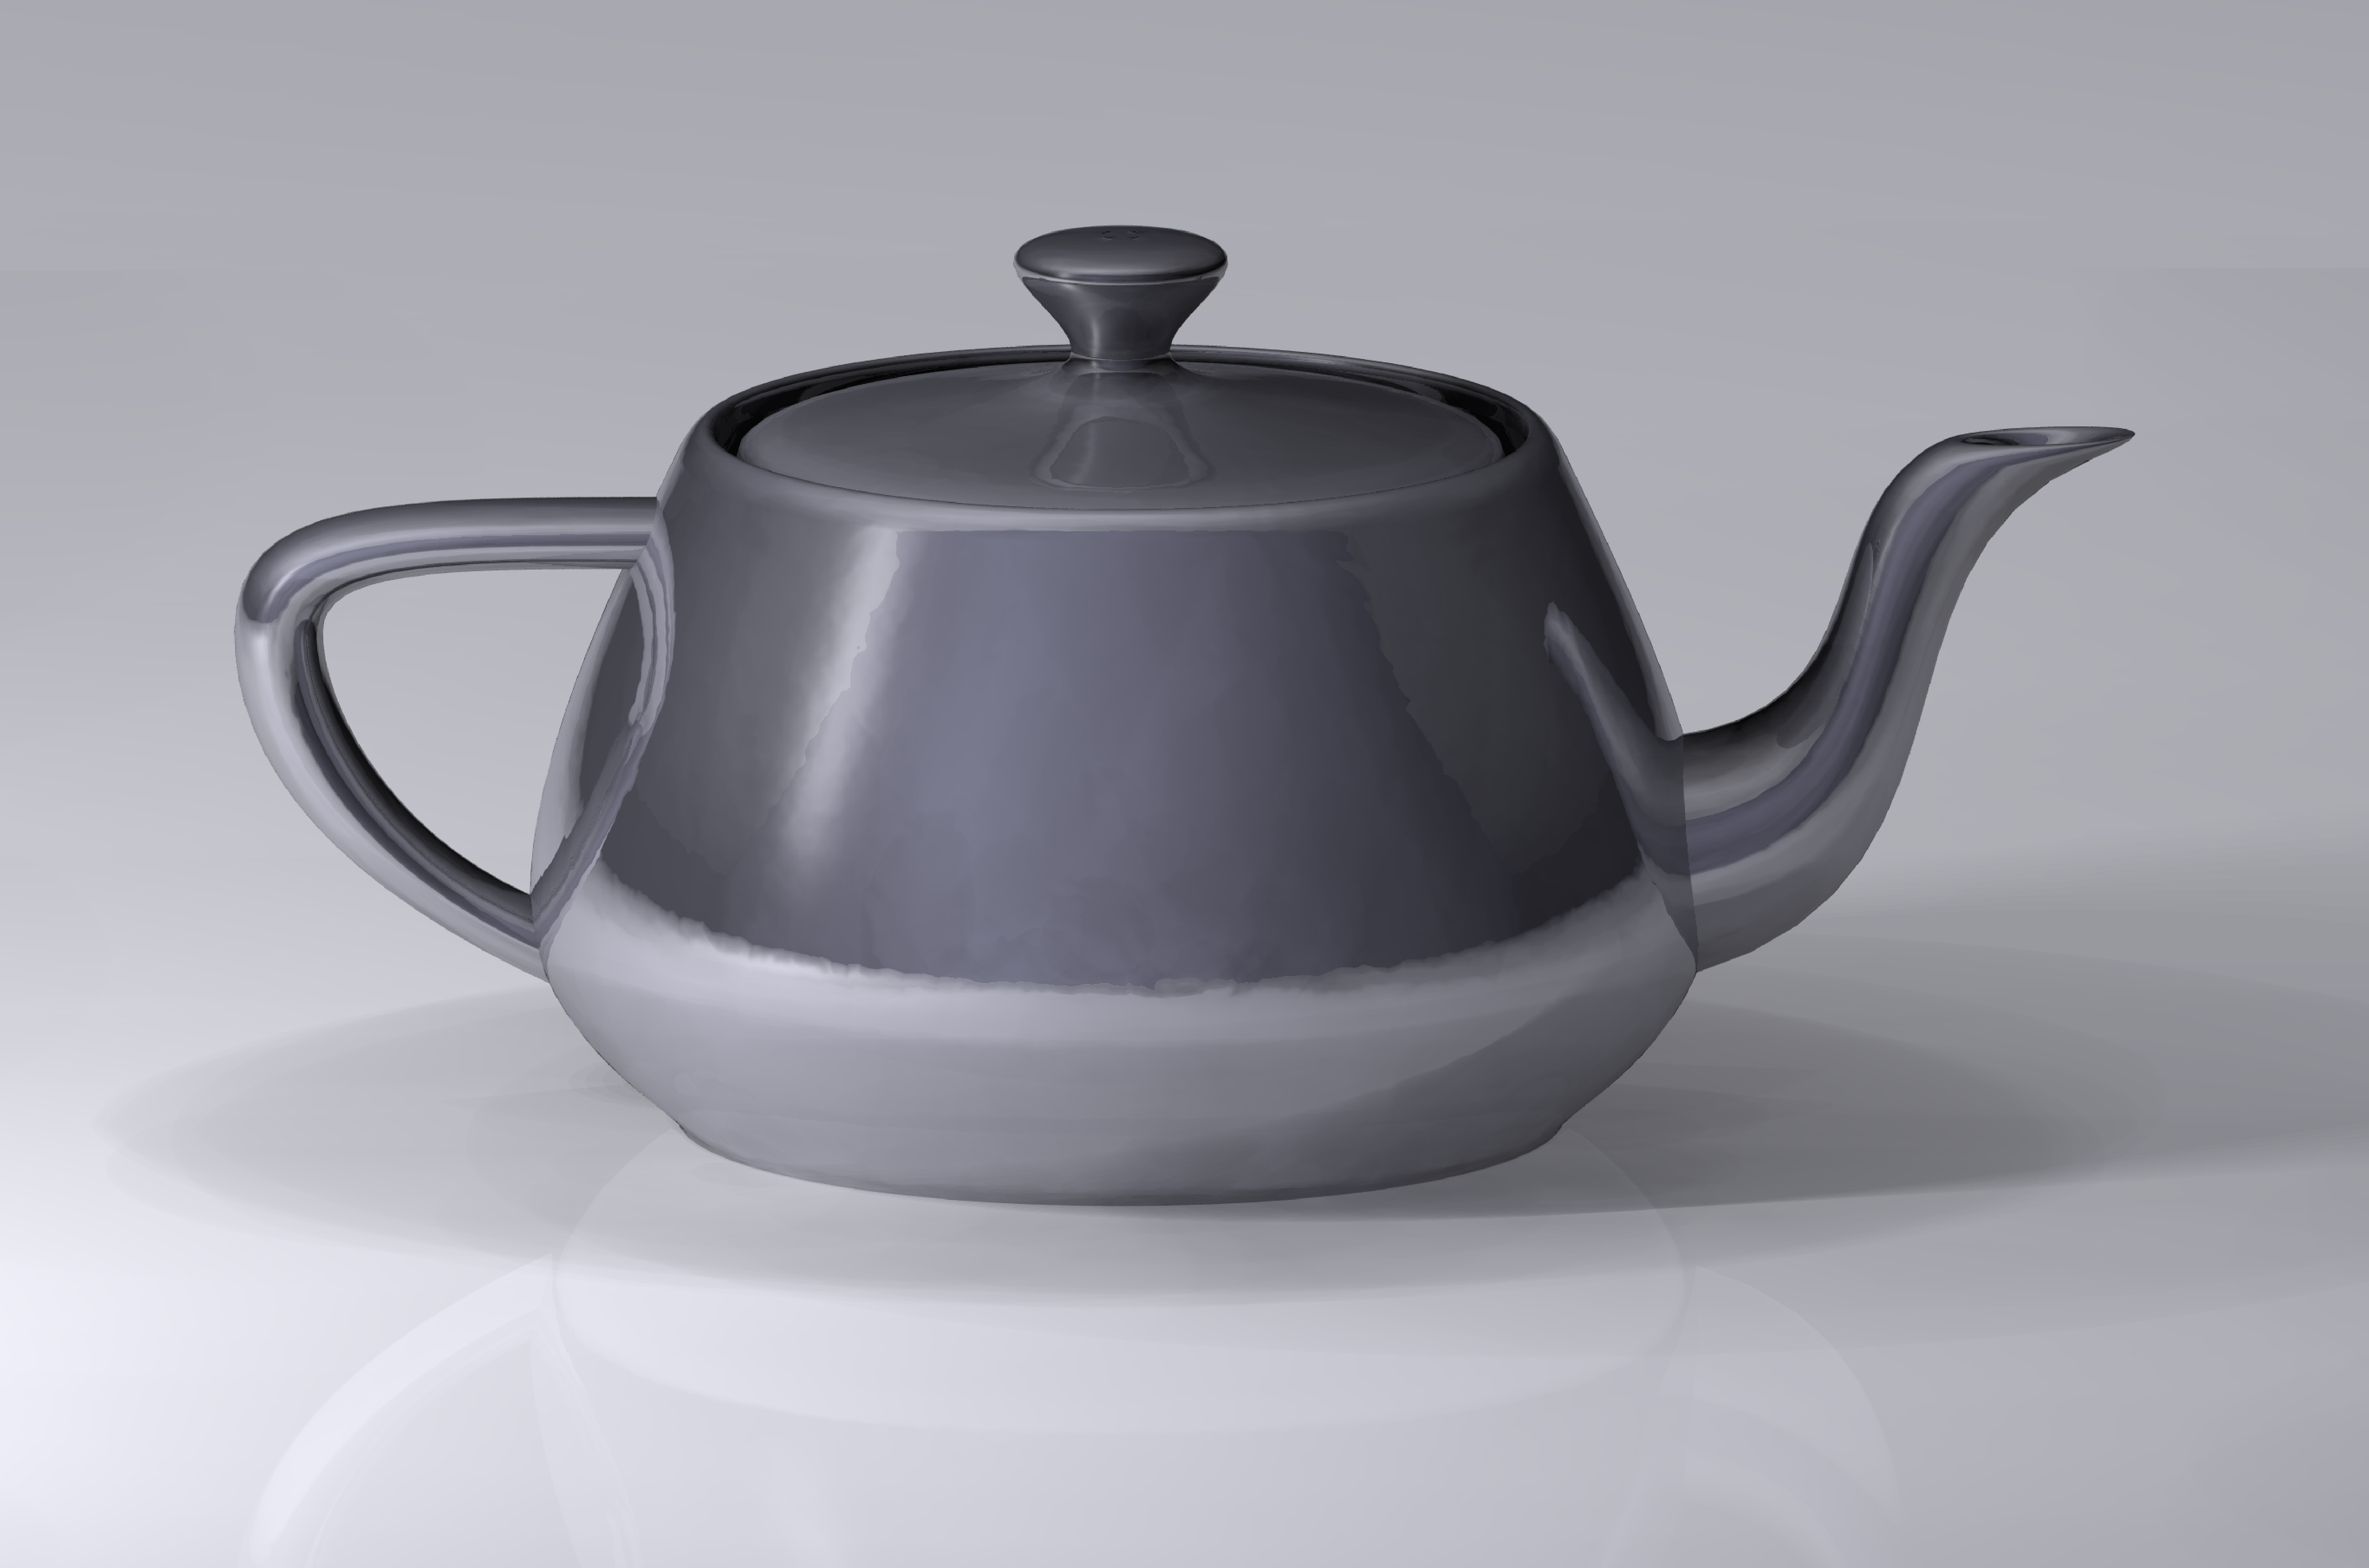
\includegraphics[width=0.7\textwidth]{figs/appendix/utah_teapot}
\caption{Lorem ipsum dolor sit amet}
\label{appendix:fig:utah_teapot}
\end{figure}


\listoffigures
\addcontentsline{toc}{chapter}{List of Figures}
\listoftables
\addcontentsline{toc}{chapter}{List of Tables}
\acknowledgments
\cv

\end{document}
